\section{Evaluation}
\label{sec:exp}


We evaluate \name on two VLM backbones, Qwen3-VL-8B~\cite{bai2025qwen3vl} and InternVL3.5-4B~\cite{wang2025internvl35}, using Qwen3-VL-8B as the default. As a plug-and-play token allocation framework, \name complements existing video RAG systems rather than replacing them. We evaluate its effectiveness on two retrieval pipelines:
(i) \textit{Embedding-based RAG}, which indexes video frames sampled at 1 FPS alongside temporally aligned subtitles, using SigLIP~2~\cite{siglip2} and BGE~\cite{bge} to score their respective relevance to the query; and
(ii) \textit{Graph-based RAG}, built on VideoRAG~\cite{ren2025videorag}, which retrieves related visual and textual evidence through a graph structure. In both cases, \name allocates a shared token budget across the retrieved evidence without modifying the underlying retrieval pipeline.

 % As such methods oftentimes retrieve top k graph nodes represented by text or frames ~\name can easily allocate over these nodes. We report prefill compute (TFLOPs) and accuracy as our main metrics, where TFLOPs can be controlled through a token budget. TFLOPs are summed over every model call that a method makes for a question, including frame scorers and planning calls, which places single-call and multi-call methods on one scale. Experiments were run on NVIDIA A100 GPUs. Due to space limitations further implementation details, hyperparameter values, and a sensitivity analysis are provided in the supplementary material.

\paragraph{Benchmarks.} 

We evaluate on three widely used single-turn, multiple-choice video understanding benchmarks and one multi-turn, open-ended benchmark:
\begin{itemize}
\item \textbf{MLVU}~\cite{zhou2024mlvu}: 2,174 multiple-choice questions across 1,242 videos from 3 minutes to 2 hours, spanning topic reasoning, anomaly recognition, needle QA, ego reasoning, plot QA, action order, and action count.

\item \textbf{LongVideoBench (LVB)}~\cite{wu2024longvideobench}: 1,337 multiple-choice questions across 752 videos from 8 seconds to 1 hour, covering 17 perception (e.g., single-scene events, objects, attributes) and relation (e.g., cross-scene order, tracking, attribute changes) tasks.

\item \textbf{Video-MME}~\cite{fu2024videomme}: 2,700 multiple-choice questions across 900 videos, divided into short ($<$2 min), medium (4--15 min), and long (30--60 min) subsets, spanning 12 tasks across perception, reasoning, OCR, and counting.

\item \textbf{MT-Video-Bench (MTVB)}~\cite{mtvideobench2025}: 1,000 open-ended dialogues (5--8 turns) across 135 videos from 20 seconds to 41 minutes, covering object reference, memory recall, content summary, and proactive interaction. Open-ended responses are scored using an LLM judge (Gemini 3.8 Flash) against a provided answer checklist.
\end{itemize}


\paragraph{Baselines.}
We compare \name against uniform sampling and five recent frame selection and token allocation methods, all operating under the same token budget. 
\begin{itemize}
\item \textbf{Top-K}: Retrieves the $K$ frames with the highest query--frame semantic similarity scores.

\item \textbf{FOCUS}~\cite{zhu2026focus}: Selects $K$ frames through multi-armed bandit exploration over temporal clips.

\item \textbf{Q-Frame}~\cite{zhang2025qframe}: Samples frames according to query relevance and allocates tokens across high-, medium-, and low-resolution tiers with a 2:1:1 budget ratio.

\item \textbf{QuoTA}~\cite{luo2025quota}: Rewrites queries into relevant entities and uses a VLM to score each frame by its likelihood of containing those entities. It then allocates tokens proportionally to the scores and downsamples tokens of each frame to a particular resolution.

\item \textbf{AdaAlloc}~\cite{an2026adaalloc}: Uses an agent to plan how to distribute the budget between low- and high-resolution frame tiers.
\end{itemize}
For multi-turn evaluation, we enable KV-cache reuse whenever a method selects evidence that exactly matches previously prefilled content: Top-K and FOCUS reuse previously seen frames, while Q-Frame and AdaAlloc reuse frames only at matching resolutions. QuoTA does not support this reuse because it downsamples tokens to variable amounts, which makes reuse impossible.


\paragraph{Metrics.}
We report answering accuracy and inference compute (TFLOPs), with the latter controlled through the token budget. To ensure a fair comparison between single- and multi-call methods, we account for prefill compute across all model calls, including auxiliary frame scoring and planning calls. Experiments are conducted on A100 GPUs. Additional implementation details, hyperparameters, and sensitivity analyses are provided in the supplementary material.
% \paragraph{Baselines.} We compare \name against uniform sampling and several state-of-the-art baselines that decide which frames from our RAG system reach the VLM and how many tokens each frame receives.
% \begin{itemize}
%   \item Top-K: Selects the top K frames with the highest semantic similarity scores. Across multi-turn Q\&A we implement it to skip prefilling already seen frames from previous turns.
%   \item FOCUS~\cite{zhu2026focus}: Selects K frames by multi-armed bandit exploration over temporal clips. Similar to Top-K it skips prefilling already seen frames across turns.
%   \item Q-Frame~\cite{zhang2025qframe}: Samples frames with a probability proportional to query relevance and bins them in three tiers in a 2:1:1 ratio of the token budget: the top-ranked frames at high resolution, the next at medium resolution, and the rest at low resolution. We modify it to skip prefilling of already seen frames of the same exact resolution.
%   \item QuoTA~\cite{luo2025quota}: Rewrites the query as a list of relevant entities, before using a VLM to score each frame based on the probability of containing the entity. Each frame then receives a share of the token budget in proportion to its score, then its tokens are downsampled towards it. As it downsamples from the entire token set, it cannot skip prefilling of any frames across turns.
%   \item AdaAlloc~\cite{an2026adaalloc} (contemporary): Lets an agent plan how to split a token budget between a low-resolution tier and a high-resolution tier. We modify it to skip prefilling of frames that exactly match the resolution tier.
% \end{itemize}

\subsection{Main Results}
\label{sec:exp-main}

\paragraph{\name achieves the Pareto frontier across single-turn video understanding.} 
As shown in \cref{tab:main}, \name achieves the highest overall accuracy across all three benchmarks and both VLM backbones. With Qwen3-VL-8B, it improves over Top-K by 2.2, 2.6, and 4.2 percentage points on MLVU, LVB, and Video-MME, respectively, at comparable compute. The gains are particularly pronounced on long videos: on the long subset of Video-MME, \name improves accuracy from 63.6\% to 71.7\% with nearly identical TFLOPs. QuoTA achieves competitive accuracy but incurs 2.8--3.4$\times$ higher compute due to its VLM-based frame scoring. These trends generalize to InternVL3.5-4B, where \name improves over Top-K by 0.5--3.5 points. Furthermore, \name consistently achieves favorable accuracy--compute trade-offs across multiple token budgets (\cref{fig:multiturn}a).


When integrated with VideoRAG, \name improves accuracy by 0.4 and 2.2 percentage points on MLVU and Video-MME, respectively, by allocating tokens across more frames at comparable compute, while accuracy decreases by 0.7 points on LVB. These results demonstrate that \name complements existing RAG designs.

% As shown in \cref{tab:main}, \name attains the best accuracy on all three benchmarks, improving over all compute-matched baselines by 0.9--7.2 points with Qwen3-VL-8B and by 0.1--6.5 points with InternVL3.5-4B. QuoTA is the only baseline that approaches this accuracy, yet its VLM-based frame scorer requires 2.8--3.4$\times$ more TFLOPs. \name also improves the accuracy of VideoRAG by X points. These gains hold across multiple token budgets (\cref{fig:multiturn}a).

\begin{figure}[t]
  \centering
  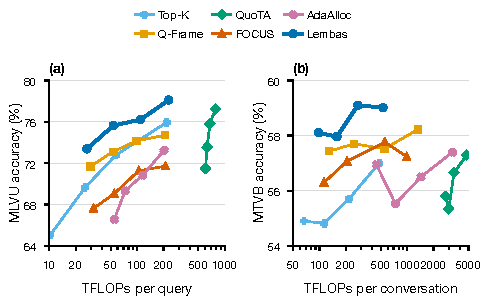
\includegraphics[width=\linewidth]{fig/tflops_pair.pdf}
  \caption{\name achieves the compute-to-accuracy Pareto frontier across (a) single-turn and (b) multi-turn video understanding.
  }
  \label{fig:multiturn}
\end{figure}

\paragraph{\name achieves the Pareto frontier across multi-turn video understanding.} 
As shown in \cref{fig:multiturn}b, \name outperforms all baselines by 0.3--1.5 percentage points while requiring 1.7--17.3$\times$ fewer TFLOPs. Unlike prior methods that reuse only previously selected frames or exact resolution matches, \name incrementally prefills only tokens not already present in the KV cache. This finer-grained reuse substantially reduces redundant computation across conversational turns while respecting answer accuracy.


\paragraph{\name introduces negligible compute overhead.}
The combined compute of semantic similarity search using FAISS~\cite{faiss}, iterative water-filling, and token pruning is below 0.001 TFLOPs per query, negligible compared with VLM prefill compute. 


% \begin{figure}[t]
%   \centering
%   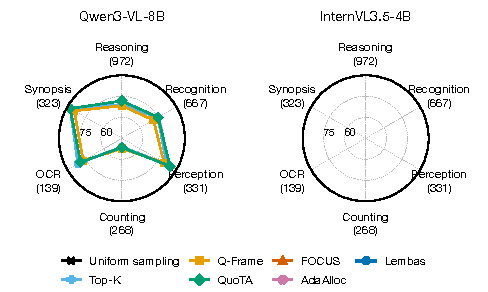
\includegraphics[width=\linewidth]{fig/videomme_radar.pdf}
%   \caption{\TODO{}}
%   \label{fig:radar}
% \end{figure}


\begin{table}[t]
  \centering
  \footnotesize
  \renewcommand{\arraystretch}{1.2}
  \settowidth{\splitw}{Medium}%
  \newcommand{\na}{--}
  \newcommand{\abltab}{%
  \begin{tabular}{l<{\hspace{5pt}} c VVVV}
    \toprule
    Method & TFLOPs $\downarrow$
      & \multicolumn{4}{c}{%
        \begin{tabular}{@{}VVVV@{}}
          \multicolumn{4}{c}{Video-MME (w/ subtitles) $\uparrow$} \\
          \cmidrule(lr){1-4}
          Overall & Short & Medium & Long \\[2.6pt]
        \end{tabular}} \\
    \specialrule{\lightrulewidth}{\aboverulesep}{0pt}
    \rowcolor{oursbg}\textbf{\name}                 & 232 & \textbf{77.3} & \textbf{83.6} & \textbf{76.8} & \textbf{71.7} \\
    \hspace{0.5em}w/o text allocation      & 226 & 73.7 & 81.9 & 74.9 & 64.4 \\
    \hspace{0.5em}w/o diversity term            & 226 & 76.6 & 82.4 & 76.4 & 70.8 \\
    \bottomrule
  \end{tabular}}%
  % Equal gaps that make the table exactly \columnwidth (12 column sides).
  \sbox0{\setlength{\tabcolsep}{0pt}\abltab}%
  \setlength{\tabcolsep}{\dimexpr(\columnwidth-\wd0)/11\relax}%
  \xdef\ablsep{\the\tabcolsep}% Table 3 reuses this gap, so both tables start at the same indent
  \abltab
  \caption{Ablation studies across single-turn Q\&A.}
  \label{tab:ablation}

  \vspace{8pt}  % Tables 2 and 3 share one float so that both stay in this column

  \centering
  \footnotesize
  \renewcommand{\arraystretch}{1.2}
  % Same side gap as Table 2 (\ablsep); the two number columns share the remaining width.
  \setlength{\tabcolsep}{\ablsep}%
  \settowidth{\dimen0}{\hspace{0.5em}w/o incremental allocation}%
  \dimen2=\dimexpr(\columnwidth-5\tabcolsep-5pt-\dimen0)/2\relax
  \begin{tabular}{l<{\hspace{5pt}} >{\centering\arraybackslash}p{\dimen2} >{\centering\arraybackslash}p{\dimen2}}
    \toprule
    Method & TFLOPs $\downarrow$ & MTVB $\uparrow$ \\
    \specialrule{\lightrulewidth}{\aboverulesep}{0pt}
    \rowcolor{oursbg}\textbf{\name}             & 275 & 58.5 \\
    \hspace{0.5em}w/o attention refinement       & 315 & 57.4 \\
    \hspace{0.5em}w/o incremental allocation & 687 & \textbf{59.1} \\
    \bottomrule
  \end{tabular}
  \caption{Ablation studies across multi-turn Q\&A.}
  \label{tab:multiturn}
\end{table}

\paragraph{Performance breakdown.}
We ablate the key components of \name in \cref{tab:ablation,tab:multiturn}. On Video-MME, removing subtitle allocation decreases overall accuracy by 3.6 points, with a particularly large 7.3-point drop on long videos. Even without subtitle allocation, \name outperforms all similarly budgeted, non-agentic frame selection baselines by 0.6--3.6 points. Removing the diversity term reduces accuracy by 0.7 points, confirming the benefit of accounting for redundant evidence during allocation.

For multi-turn conversations, removing attention refinement decreases accuracy by 1.1 points while increasing prefill compute from 275 to 315 TFLOPs, demonstrating that attention to cached evidence improves subsequent allocations. Disabling incremental allocation increases compute from 275 to 687 TFLOPs (2.5$\times$), with only a 0.6-point accuracy increase. These results show that attention refinement improves evidence selection, while incremental allocation is the primary driver of multi-turn compute savings. 

Additional hyperparameter sensitivity analyses are provided in the supplementary material.
